\section{Introduction}

%% Background
In this paper, we study streaming analytics in the wide area, where the data
generating sites are different from data processing sites. Such data is most
valuable if we can transport, distill and analyze in real time. For example, a
content distribution network (CDN) analyzes the logs from geo-distributed
infrastructure to optimize content placement. Recently, the emerging class of
Internet of Things (IoT) applications makes the wide-area streaming analytical
workload even more important. Large cities such as New York, Beijing and Seattle
have deployed millions of cameras for traffic
control~\cite{london.surveillance,skynet}. Our buildings are increasingly
equipped with a wide variety of sensors to improve building energy use, occupant
comfort, reliability and maintenance~\cite{krioukov2012building}.

While existing stream processing systems, such as Spark
Streaming~\cite{zaharia2013discretized}, and specialized analytical engines,
such as VideoStorm~\cite{zhang2017live}, are capable of handling large streams
of data, they are designed to work within a single cluster. Within a single
cluster, there is sufficient bandwidth between worker nodes; in contrast the
wide area has scarce and variable bandwidth~\cite{hsieh17gaia,
  vulimiri2015global}. Back-hauling all the data across the wide-area is neither
viable nor efficient. The growth of the wide-area bandwidth has been
decelerating for many years~\cite{global2016telegeography} while the traffic
grows at a staggering rate~\cite{index2013zettabyte}. On the efficiency side,
raw data often contains large and less relevant details that can be aggregated,
pruned or compressed~\cite{rabkin2014aggregation}.

\fixme{This paragraph is rough}. Talk about local computation. Recent researches
on WAN-aware systems pushes computation to the
edge~\cite{satyanarayanan2009case, rabkin2014aggregation, pu2015low}. However,
in many cases, transmitting the data back is
unavoidable. Wireless~\cite{zhang2015design, abari2017enabling}.
% could improve efficiency (such as GDA pushes queries out; cloudlet
% etc). However, we still need data transmission for cloud off-loading or
% aggregation purpose.

When facing insufficient bandwidth, application developers need to make a
decision within the design space of data freshness and data fidelity
(\autoref{fig:intro}):

\begin{figure}
  \centering
  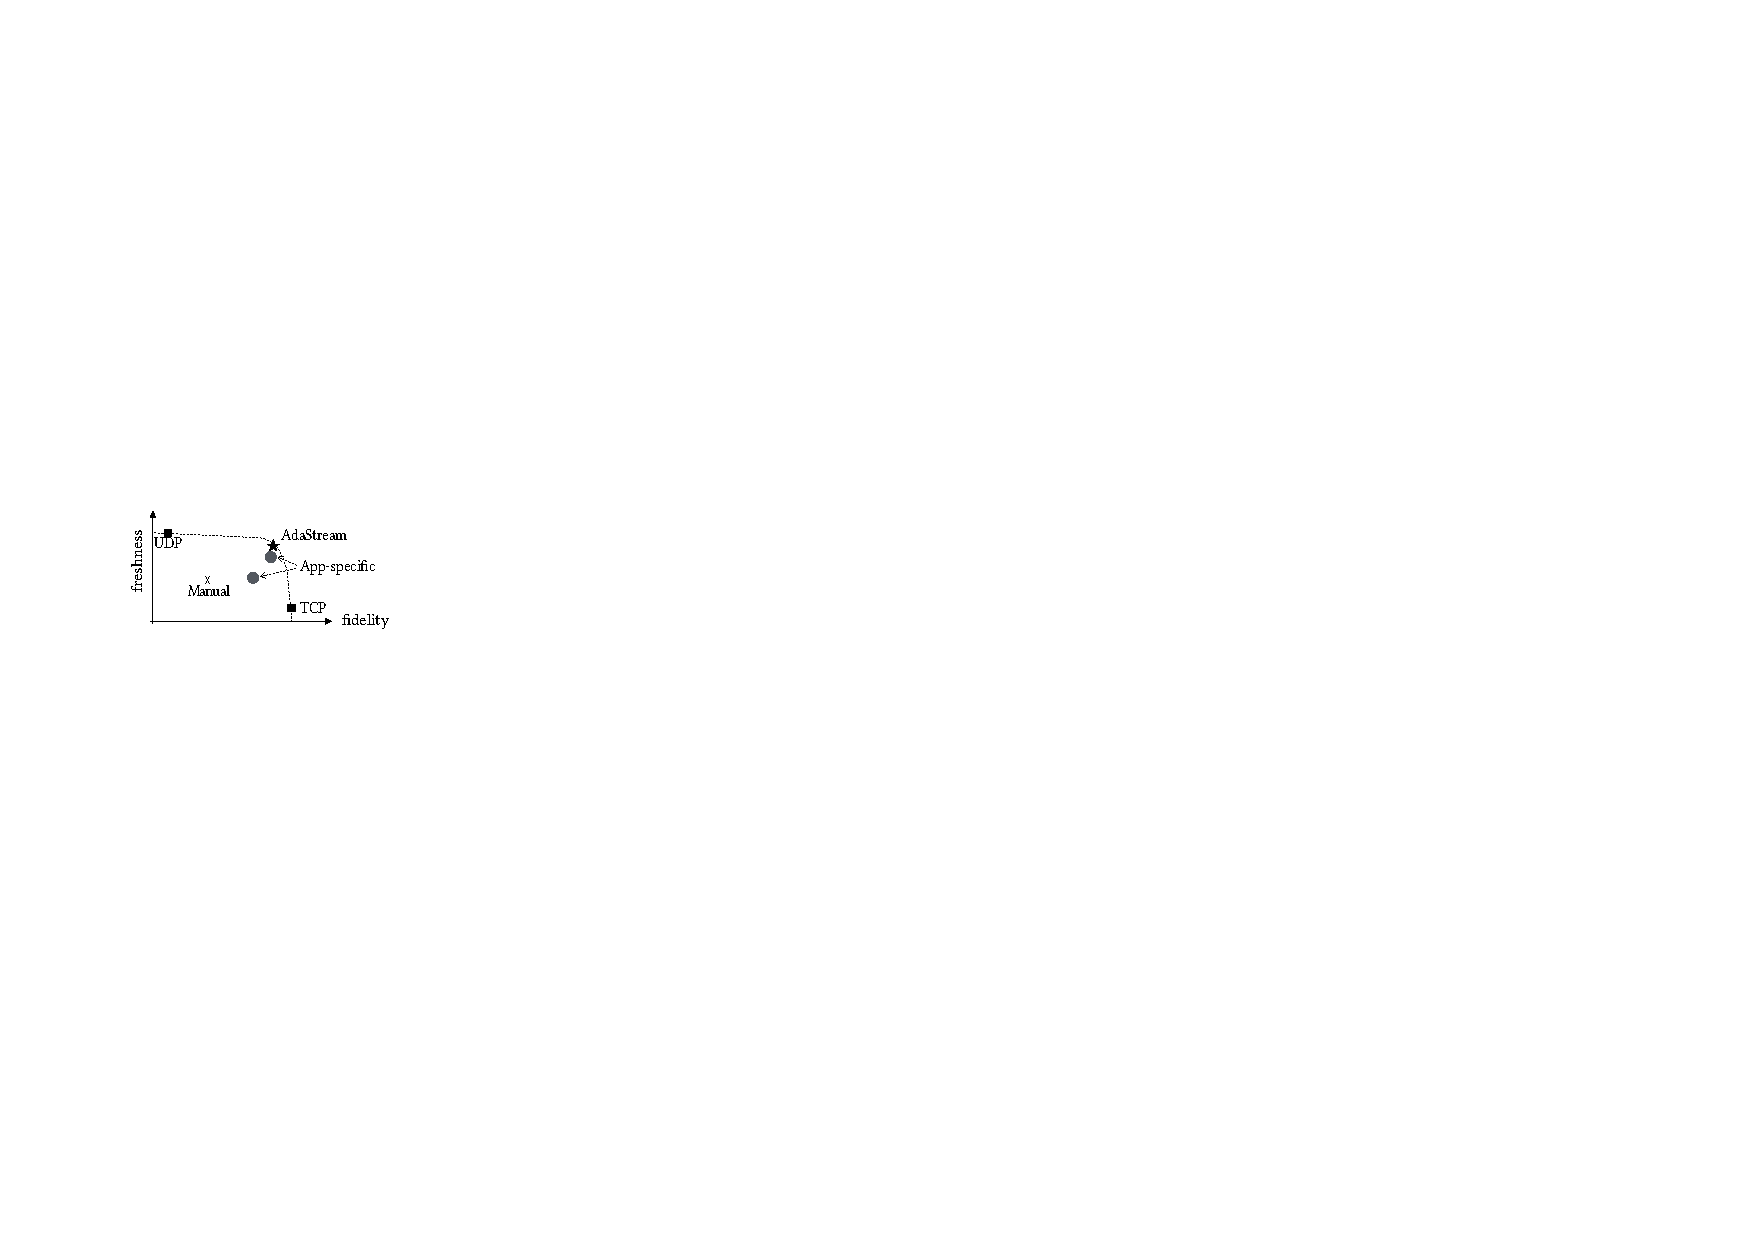
\includegraphics[width=0.9\linewidth]{figures/intro.pdf}
  \caption{The trade-off space between data freshness and data fidelity when
    facing insufficient bandwidth.}
  \label{fig:intro}
  \vspace{-1em}
\end{figure}

(i) Existing transport protocols often choose one extreme point in the design
space. Building applications with TCP ensures a reliable delivery of the data
but the backlogged data will increase application latency. Building applications
with UDP minimizes latency by sending packets as fast as possible, but the
uncontrolled packet loss along the network may devastate the application.

(ii) Manual policies, such as sampling, can trade data fidelity for
freshness~\cite{rabkin2014aggregation}. But these policies are often developer
heuristics without measurements backing up. An accurate policy often requires
extensive developer efforts or domain expertise. These policies, in practice,
often provide sub-optimal performance in both freshness and fidelity.

(iii) Application-specific optimizations do not generalize. The trade-off
strategy designed to work well for one application under one condition renders
sub-optimal performances in a different scenario. For example, video-on-demand
was designed for human consumption, and adaptations have focused on Quality of
Experience (QoE)~\cite{yin2015control}. Humans prefers smoothness over image
quality. This limits potential dimensions in the adaptation space, i.e., they
need to maintain 25 frames per seconds (FPS).

In this paper, we present \sysname{}, a stream processing system for the wide
area that addresses the bandwidth limitations with a system-level solution. At
the core, \sysname{} integrates application adaptation as a first-class
abstraction within the stream processing model. Similar to other operators such
as \texttt{map} or \texttt{window}, our proposed \maybe{} operator is part of
the stream processing application. The operator take a list of values as a knob
and a function that transforms an input stream into a degraded stream. By
specializing the function, we've built a library of degradation operators for
common data types, such as \texttt{maybe\_head} for a list or
\texttt{maybe\_downsample} for images.

Our APIs offer a number of advantages over existing approaches. First,
developers are not assume to be experts in the application domain. Instead of
writing exact policies, developers only need to hint at potential
operations. For example, while a developer may not understand how downsampling
the video affects data rate or object detection accuracy, she can express the
downsample operation with a few resolution options. Second, \sysname{}'s APIs
are modular, extensible and allow easy integration. Custom functions from
external libraries be embedded inside the operator. The similarity with other
operators makes it easy to integrate with existing stream processing systems.
We name our approach \textit{structured adaptation} to contrast from existing
adaptations using ad-hoc policies.

\sysname{} uses a data-driven approach to learn the application performance for
different levels of degradation. The combination of \maybe{} operators form a
\textit{configuration} that affects bandwidth demand and application
accuracy. By evaluating over a representative training dataset and an
application-specific accuracy measure, \sysname{} explores the configuration
space automatically to learn a Pareto-optimal adaptation strategy. The strategy,
or \textit{profile}, contains configurations that offer the highest accuracy
with a given bandwidth constrain. \sysname{} performs both offline and online
profiling. Profiling can be expensive over the entire configuration space. We
speed up the process with parallelism. For some applications, online profiling
is needed to alleviate \textit{model drift}, where a previously learned profile
doesn't match new data. \sysname{} addresses model drift with online profiling.
To further speed up the online profiling, we use the offline profile information
for scheduling and avoiding full profiling.

At runtime, we use the profiles to adapt the application execution, such as the
data rate matches the available bandwidth. Our rate adaptation employs a novel
probe-based control that allows fine-tuning the egress data rate. When multiple
streams share the same bottle-neck link, our system is able to allocate
bandwidth resources to maximize the minimal accuracy, achieving
utility-fairness.

To evaluate \sysname{}, we've built three streaming applications: pedestrian
detection (PD), augmented reality (AR) and a distributed Top-K (TK) analysis. We
use real-world data to evaluate these applications for our profiling tool and
runtime systems. The evaluation results and our contributions are summarized as
follows:

\begin{itemize}[leftmargin=16pt]
\item We design and implement \sysname{}, the first stream processing system
  that simultaneously achieves low latency and high accuracy.
\item We propose to integrate adaptation as a first-class abstraction in stream
  processing: it requires minimal developer efforts and the profile are accurate
  with a data-driven approach.
\item We build three real-world applications and our evaluation shows that
  \sysname{} generates Pareto-optimal profiles with precision and fine
  granularity for all three applications evaluate their behavior under different
  scenarios.
\item We propose a rate adaptation scheme that adapts the application data to
  available bandwidth, with a goal of minimizing the latency. Our evaluations
  shows that we can achieve sub-second latency and nominal accuracy drop.
\end{itemize}

%%% Local Variables:
%%% mode: latex
%%% TeX-master: "sosp17"
%%% End:

%% LocalWords: VideoStorm, analytics, CDN, IoT
